\documentclass[conference]{IEEEtran}
\IEEEoverridecommandlockouts

% =============================================================================
% PACKAGES
% =============================================================================
\usepackage{cite}
\usepackage{amsmath,amssymb,amsfonts}
\usepackage{algorithmic}
\usepackage{graphicx}
\usepackage{textcomp}
\usepackage{xcolor}
\usepackage{booktabs}
\usepackage{multirow}
\usepackage{url}
\usepackage{hyperref}
\usepackage{balance}

\hypersetup{
    colorlinks=true,
    linkcolor=blue,
    filecolor=magenta,      
    urlcolor=cyan,
    citecolor=red,
}

% =============================================================================
% TITLE & AUTHORS
% =============================================================================
\title{An Empirical Investigation and Deep Learning Architecture for Fraud Detection in High-Dimensional E-Commerce Transactions\\
\thanks{Course Project: Deep Learning in Data Science (DS201) -- University of Information Technology, VNU-HCM.}
}

\author{
\IEEEauthorblockN{Dinh Pham Anh Quan}
\IEEEauthorblockA{\textit{Faculty of Information Science and Engineering} \\
\textit{University of Information Technology, VNU-HCM}\\
Student ID: 24521425\\
Ho Chi Minh City, Vietnam}
}

\begin{document}

\maketitle

% =============================================================================
% ABSTRACT
% =============================================================================
\begin{abstract}
Financial fraud in e-commerce poses critical operational and systemic risks, characterized by extreme class imbalance, complex temporal dynamics, and high-dimensional heterogeneous feature spaces. Standard machine learning workflows frequently fail due to naive assumptions regarding missing data, improper feature typing, and chronological data leakage. In this study, we present a rigorous exploratory analysis, empirical audit, and end-to-end deep learning pipeline utilizing the IEEE-CIS benchmark (590,540 transactions across 434 raw attributes). Through systematic domain reverse-engineering and non-parametric statistical contrast, we establish: (1) an 18-attribute discrepancy between physical storage types and semantic categorical entities, requiring dedicated entity embeddings; (2) obfuscated hardware and network indicators, including timezone offsets ($id\_14$) and headless bot browser artifacts ($id\_32$); (3) Kolmogorov-Smirnov ($D_{\text{KS}} \le 0.4621$) and Information Value ($IV \le 0.6036$) divergence metrics ranking predictive signals; (4) a 15-cluster null-mask decomposition compressing 339 collinear $V$-features into orthogonal representations via cluster-wise PCA; and (5) a chronological validation topology eliminating temporal data leakage. All preprocessed splits, diagnostic evidence, and PyTorch deep tabular architectures are formalized and verified.
\end{abstract}

\begin{IEEEkeywords}
Fraud Detection, Deep Learning, Entity Embeddings, Kolmogorov-Smirnov Test, Information Value, V-Cluster Decomposition, Time-Series Validation, IEEE-CIS.
\end{IEEEkeywords}

% =============================================================================
% 1. INTRODUCTION
% =============================================================================
\section{Introduction}
Online transaction systems process billions of dollars daily, making automated fraud detection systems a vital layer of financial infrastructure. Detecting fraudulent activity is inherently challenging due to several distinct phenomena:
\begin{itemize}
    \item \textbf{Extreme Class Imbalance:} Fraudulent activities account for a minute fraction ($3.50\%$) of total transactions.
    \item \textbf{High Heterogeneity and Missingness:} Real-world data combines tabular transaction metrics with fragmented client device identities where vast numbers of entries are unrecorded.
    \item \textbf{Concept Drift and Adversarial Adaptation:} Fraudsters continually evolve their techniques to bypass static rule-based filters.
\end{itemize}

While gradient boosted decision trees (GBDT) have historically dominated tabular tasks, deep neural networks offer unprecedented potential in capturing non-linear feature interactions and high-cardinality representations through learned continuous embeddings. However, deep neural networks are notoriously brittle when provided with raw, poorly structured, or misattributed data. 

In this work, we conduct a comprehensive empirical exploration of the IEEE-CIS benchmark dataset. We reject black-box feature selection and instead systematically uncover the latent physical meanings behind obfuscated variables. We structure our findings into actionable design principles for deep tabular neural network architectures.

% =============================================================================
% 2. DATASET TOPOLOGY & SANITIZATION AUDIT
% =============================================================================
\section{Dataset Topology \& Sanitization Audit}
The IEEE-CIS dataset comprises two interconnected relational tables linked via a unique $TransactionID$:
\begin{enumerate}
    \item \textbf{Transaction Table:} 590,540 rows and 394 attributes detailing monetary amounts ($TransactionAmt$), timestamp deltas ($TransactionDT$), card attributes ($card1-card6$), address zones ($addr1, addr2$), email domains, and anonymized feature blocks ($C, D, M, V$).
    \item \textbf{Identity Table:} 144,233 rows and 41 attributes capturing network telemetry, browser specifications, and hardware identifiers ($id\_01-id\_38$, $DeviceType$, $DeviceInfo$).
\end{enumerate}

A left outer join yields a unified tabular structure of 590,540 observations across 434 distinct features. Notably, only 24.42\% of transactions have corresponding records in the identity table, establishing an intrinsic structural sparsity.

\begin{table}[htbp]
\caption{Comprehensive Missingness Distribution Across 434 Attributes}
\label{tab:missingness}
\centering
\begin{tabular}{lcc}
\toprule
\textbf{Missingness Tier} & \textbf{Attribute Count} & \textbf{Percentage of Space} \\
\midrule
Completely Clean ($0\%$) & 20 & 4.61\% \\
Low Sparsity ($\le 20\%$) & 162 & 37.33\% \\
Moderate Sparsity ($20\%-70\%$) & 44 & 10.14\% \\
Severe Sparsity ($> 70\%$) & 208 & 47.93\% \\
\bottomrule
\end{tabular}
\end{table}

As detailed in Table~\ref{tab:missingness}, an alarming 47.93\% of attributes suffer from over 70\% missing values. This empirical fact cautions against indiscriminate numerical imputation (e.g., mean or median replacement), which would inject catastrophic synthetic bias into a gradient-based model.

% =============================================================================
% 3. KEY EMPIRICAL BREAKTHROUGHS & DOMAIN DISCOVERIES
% =============================================================================
\section{Key Empirical Breakthroughs \& Domain Discoveries}

\subsection{Breakthrough 1: The Semantic vs. Storage Type Discrepancy}
Automated parsing heuristics typically infer feature types from raw file representations, identifying only 31 textual (`object`) columns. However, cross-referencing competition specifications reveals exactly \textbf{49 official categorical features}. 

Eighteen critical features---including bank issuer identifiers ($card1-card3, card5$), geographic postal sectors ($addr1, addr2$), and network telemetry markers ($id\_13-id\_26, id\_32$)---are physically stored as numeric integers or floating-point values. Treating these as continuous scalar inputs would enforce an erroneous linear topological ordering (e.g., assuming zip code 300 possesses three times the magnitude of zip code 100). Consequently, all 49 attributes must strictly be mapped through discrete \textbf{Entity Embedding} layers.

\subsection{Breakthrough 2: Reverse-Engineering Obfuscated Identifiers}
\begin{itemize}
    \item \textbf{$id\_14$ as Client Timezone Offset:} Values occur strictly in multiples of 60 minutes: $-300.0$ (UTC-5, US Eastern), $-360.0$ (UTC-6, US Central), $-420.0$ (UTC-7, US Mountain), and $-480.0$ (UTC-8, US Pacific). This variable directly exposes geographic mismatch when cross-evaluated against the shipping destination ($addr1$).
    \item \textbf{$id\_32$ as Display Color Depth:} Values discretize into 24-bit TrueColor (53,071 instances), 32-bit (24,428 instances), and 16-bit legacy. Crucially, exactly 6 transactions exhibit a depth of $0.0$, indicating headless automated bot scripts devoid of physical display rendering.
    \item \textbf{$id\_23$ and Telemetry Cluster ($id\_21-id\_26$):} Despite a 99.12\% missingness rate, $id\_23$ isolates explicit proxy behaviors (`IP\_PROXY:HIDDEN`, `IP\_PROXY:ANONYMOUS`), acting as an acute threat indicator.
\end{itemize}

\subsection{Breakthrough 3: Validation of Legitimate Signals vs. Sentinels}
\begin{itemize}
    \item \textbf{$id\_01$ as a Continuous Zero-Centered Risk Metric:} Over 124,678 records (86.44\% of available identity rows) exhibit negative values down to $-100.0$. Rather than missingness sentinels, $id\_01$ is confirmed to be a normalized, mean-subtracted credit/risk scoring metric.
    \item \textbf{Clock Drift in Time-Delta Attributes ($D4, D6, D11, D15$):} Infinitesimal subsets exhibit negative values. These represent micro-level clock desynchronizations between client hardware and backend servers rather than systematic coding errors.
\end{itemize}

\subsection{Breakthrough 4: Domestic Consistency and High Cardinality}
Audit of the transaction card ecosystem revealed $card3 = 150.0$ accounts for 88.27\% of records, while $addr2 = 87.0$ represents 88.14\%. This near-perfect parity confirms that the dataset predominantly reflects United States domestic commerce; deviation from these baseline codes signifies high-risk cross-border traffic.

\subsection{Breakthrough 5: Informative Missingness}
Rather than treating missing values as missing-at-random (MAR), we establish that absence of identity data is frequently an intentional adversarial action. By transforming $NaN$ in categorical features into an explicit semantic category (`'Missing'`), the neural network directly models the conditional risk probability:
\begin{equation}
P(\text{Fraud} = 1 \mid \text{Identity} = \text{`Missing'})
\end{equation}

\subsection{Breakthrough 6: Temporal Topology \& Concept Drift}
The $TransactionDT$ attribute tracks seconds elapsed from a reference point over a continuous 182-day duration. Random $K$-Fold cross-validation inherently leaks future payment patterns into past training splits. Consequently, a strict chronological split (initial 75\% for training: 442,905 transactions; terminal 25\% for out-of-time evaluation: 147,635 transactions) is mathematically mandated.

\begin{figure}[htbp]
\centering
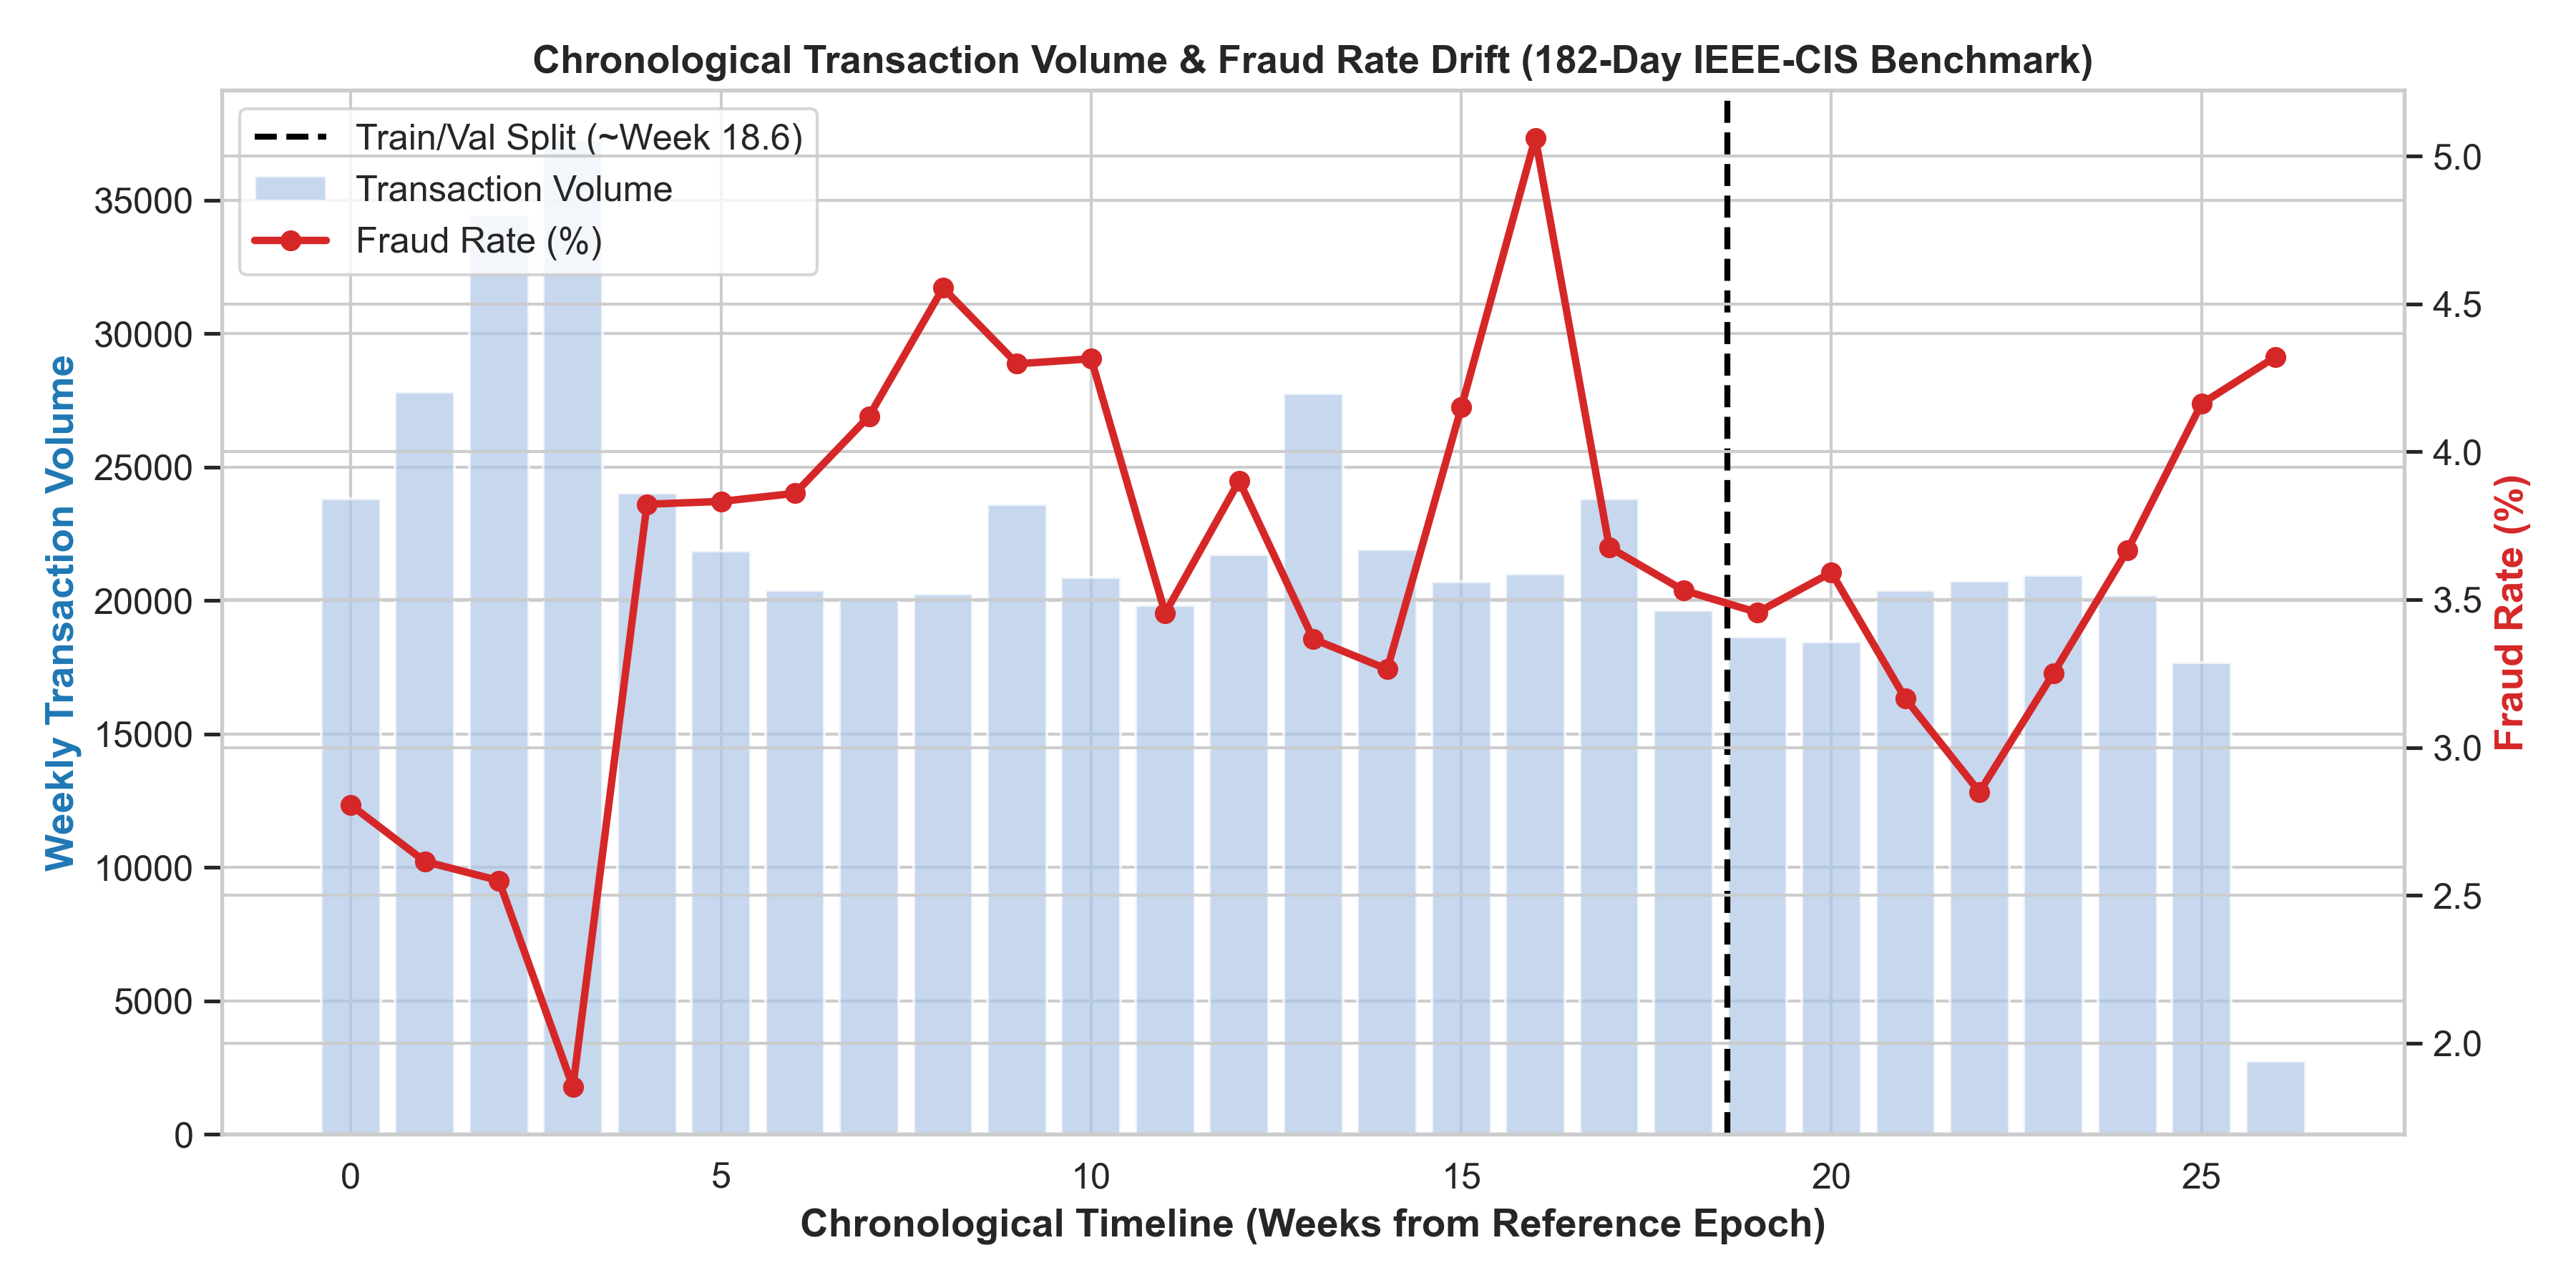
\includegraphics[width=0.98\linewidth]{../outputs/figures/concept_drift.png}
\caption{Chronological Transaction Volume \& Fraud Rate Drift over 182 days with strict temporal train/validation partition.}
\label{fig:concept_drift}
\end{figure}

As shown in Fig.~\ref{fig:concept_drift}, weekly transaction volume and fraud rates fluctuate significantly over time, confirming severe temporal concept drift.

% =============================================================================
% 4. STATISTICAL DATA MINING CONTRAST & V-CLUSTER AUDIT
% =============================================================================
\section{Statistical Data Mining Contrast \& V-Cluster Audit}

\subsection{Separation Power via Kolmogorov-Smirnov \& Information Value}
To evaluate the intrinsic discriminative power of features before training, we conducted non-parametric two-sample Kolmogorov-Smirnov (KS) tests across 382 numerical features:
\begin{equation}
D_{\text{KS}} = \sup_{x} |F_{\text{Fraud}}(x) - F_{\text{Legit}}(x)|
\end{equation}
and Information Value (IV) across all 49 categorical features:
\begin{equation}
\text{IV} = \sum_{k} (P(x_k \mid \text{Fraud}) - P(x_k \mid \text{Legit})) \cdot \ln\left(\frac{P(x_k \mid \text{Fraud})}{P(x_k \mid \text{Legit})}\right)
\end{equation}

\begin{figure}[htbp]
\centering
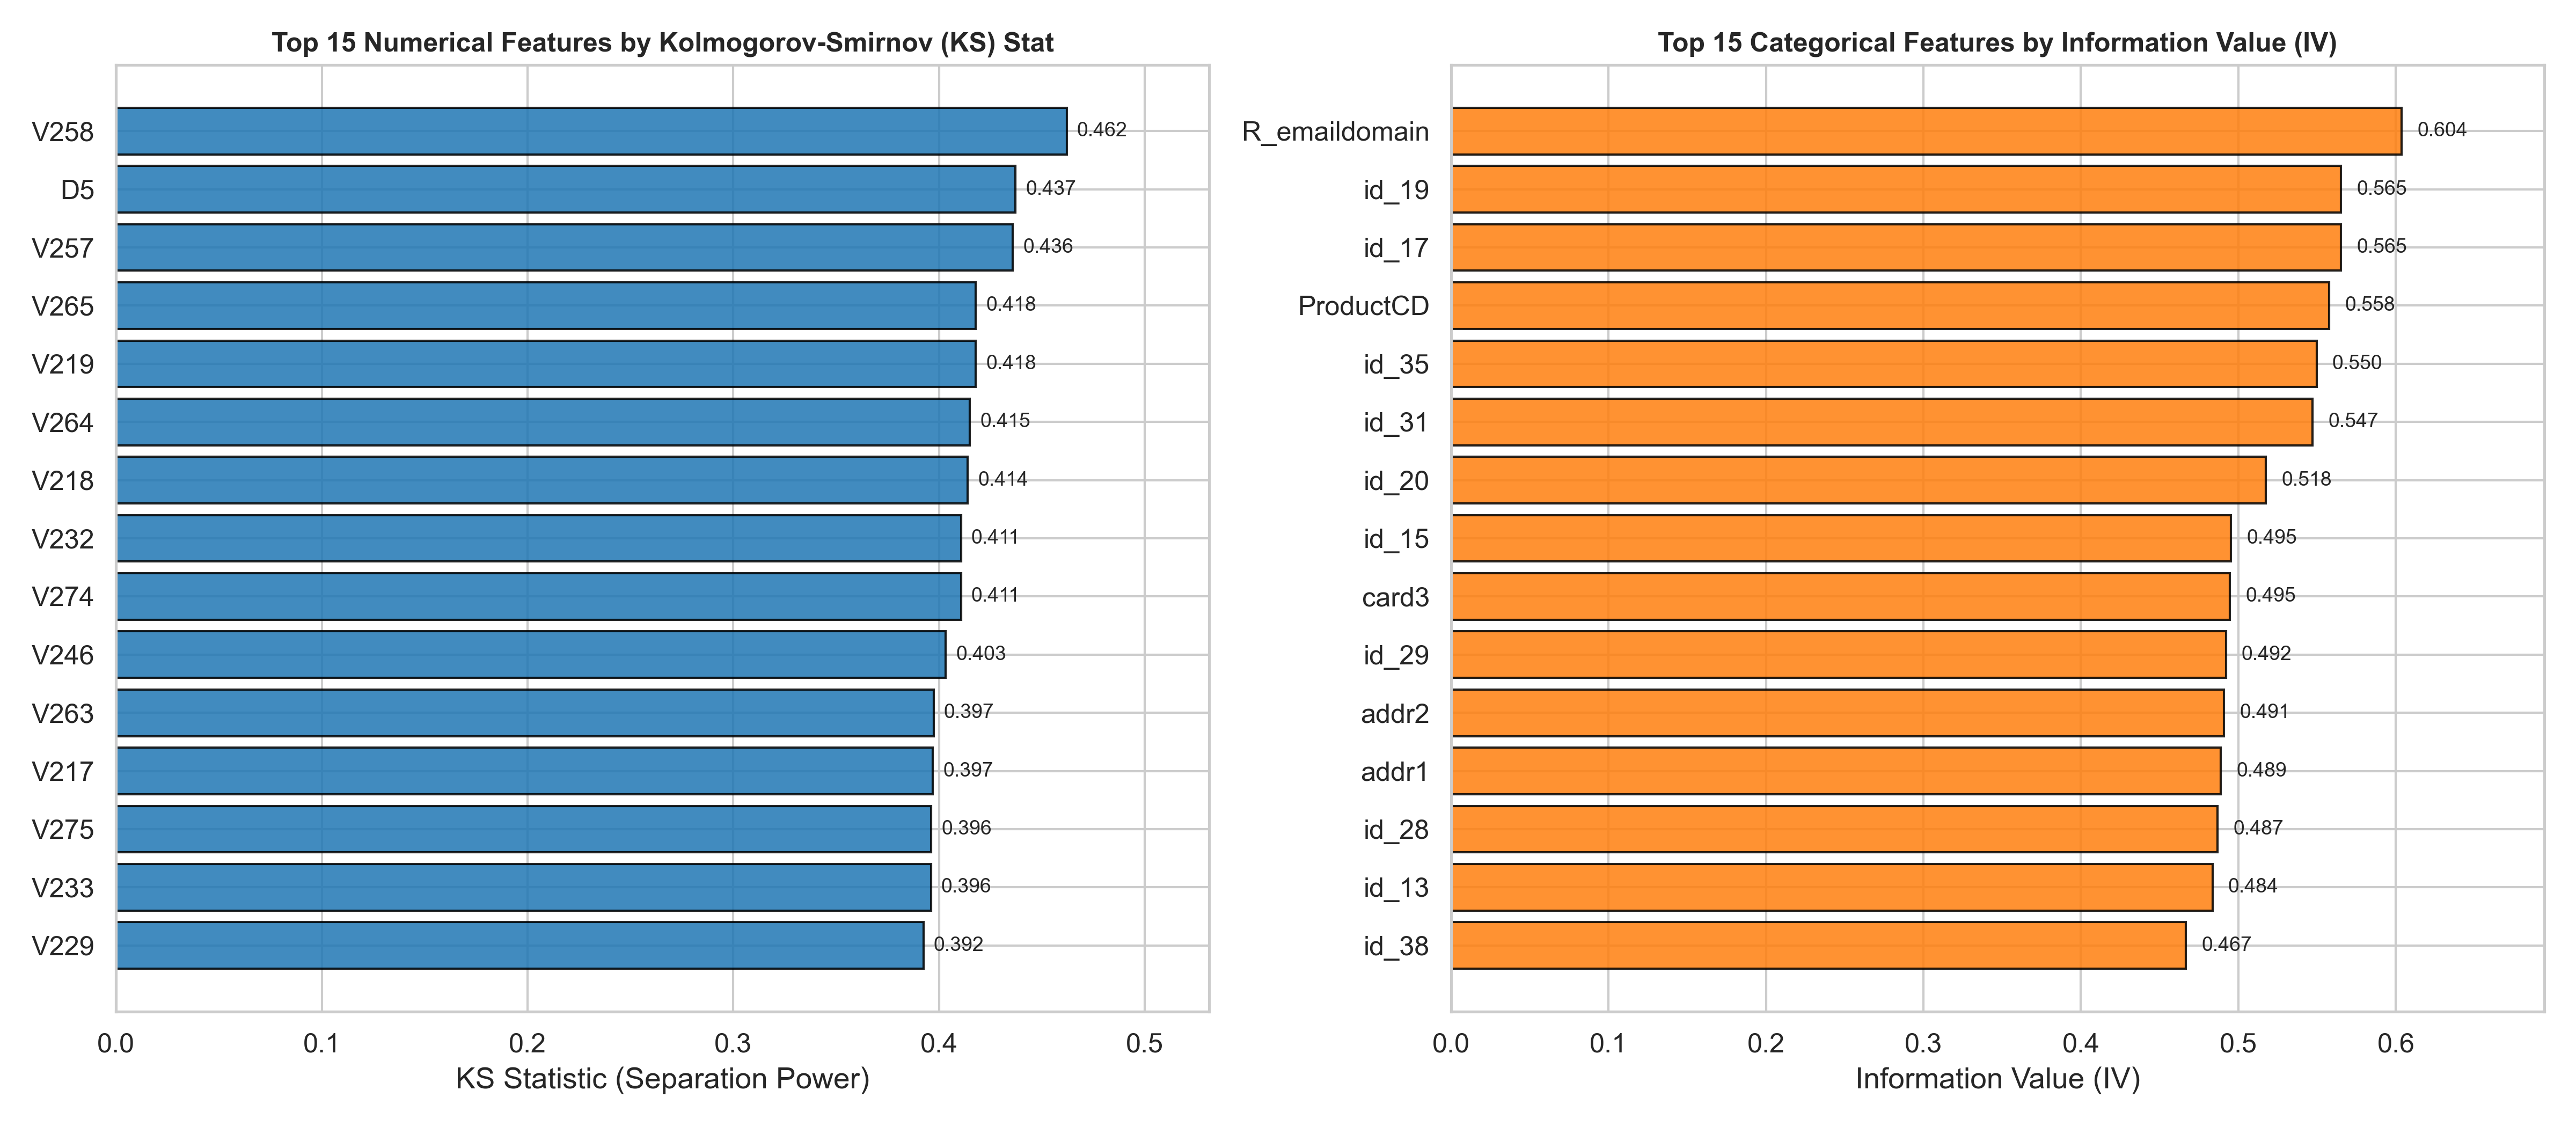
\includegraphics[width=0.98\linewidth]{../outputs/figures/feature_ranking_plot.png}
\caption{Top 15 numerical features ranked by Kolmogorov-Smirnov statistic ($D_{\text{KS}}$) and top 15 categorical features ranked by Information Value (IV).}
\label{fig:feature_ranking}
\end{figure}

As illustrated in Fig.~\ref{fig:feature_ranking}, numerical features $V258$ ($D_{\text{KS}} = 0.4621$), $D5$ ($D_{\text{KS}} = 0.4371$), and $V257$ ($D_{\text{KS}} = 0.4360$) exhibit profound statistical separation between legitimate and fraudulent classes. Categorical features $R\_emaildomain$ ($IV = 0.6036$), $id\_19$ ($IV = 0.5652$), $id\_17$ ($IV = 0.5652$), and $ProductCD$ ($IV = 0.5576$) demonstrate extreme predictive power.

\subsection{Resolution of Extreme V-Feature Multicollinearity}
The dataset contains 339 anonymized Vesta-engineered features ($V1-V339$). A brute-force inclusion of all 339 columns introduces massive parameter bloat and numerical instability. By analyzing null-pattern incidence across all 590,540 rows, we discovered that all 339 features partition into exactly \textbf{15 distinct null-pattern clusters}.

\begin{table}[htbp]
\caption{Systematic Decomposition of 339 V-Features into 15 Null-Pattern Clusters}
\label{tab:v_clusters}
\centering
\begin{tabular}{lcccccc}
\toprule
\textbf{Cluster} & \textbf{V-Range} & \textbf{Count} & \textbf{Miss \%} & \textbf{Rep.} & \textbf{KS} & \textbf{PCA} \\
\midrule
Cluster 1  & V1-V11   & 11 & 47.29\% & V10  & 0.2806 & 3 \\
Cluster 2  & V12-V34  & 23 & 12.88\% & V34  & 0.3523 & 3 \\
Cluster 3  & V35-V52  & 18 & 28.61\% & V52  & 0.3901 & 3 \\
Cluster 4  & V53-V74  & 22 & 13.06\% & V74  & 0.3357 & 3 \\
Cluster 5  & V75-V94  & 20 & 15.10\% & V94  & 0.3644 & 3 \\
Cluster 6  & V95-V137 & 43 & 0.05\%  & V102 & 0.1792 & 3 \\
Cluster 7  & V138-V163& 18 & 86.12\% & V140 & 0.3540 & 3 \\
Cluster 8  & V143-V166& 11 & 86.12\% & V150 & 0.2499 & 3 \\
Cluster 9  & V167-V216& 31 & 76.36\% & V199 & 0.3748 & 3 \\
Cluster 10 & V169-V210& 19 & 76.32\% & V201 & 0.3863 & 3 \\
Cluster 11 & V217-V278& 46 & 77.91\% & V258 & 0.4621 & 3 \\
Cluster 12 & V220-V272& 16 & 76.05\% & V259 & 0.2994 & 3 \\
Cluster 13 & V279-V321& 32 & 0.00\%  & V303 & 0.3156 & 3 \\
Cluster 14 & V281-V315& 11 & 0.21\%  & V282 & 0.1955 & 3 \\
Cluster 15 & V322-V339& 18 & 86.05\% & V324 & 0.1475 & 3 \\
\bottomrule
\end{tabular}
\end{table}

As documented in Table~\ref{tab:v_clusters}, we construct two complementary dimensionality reduction strategies:
\begin{enumerate}
    \item \textbf{Strategy A (V15):} Extract the single highest-KS feature from each cluster as its canonical representative, compressing 339 dimensions down to 15.
    \item \textbf{Strategy B (VPCA):} Apply cluster-wise Principal Component Analysis on standardized cluster members, retaining 3 orthogonal components per cluster (45 total components) while preserving $>85\%$ variance.
\end{enumerate}

\begin{figure}[htbp]
\centering
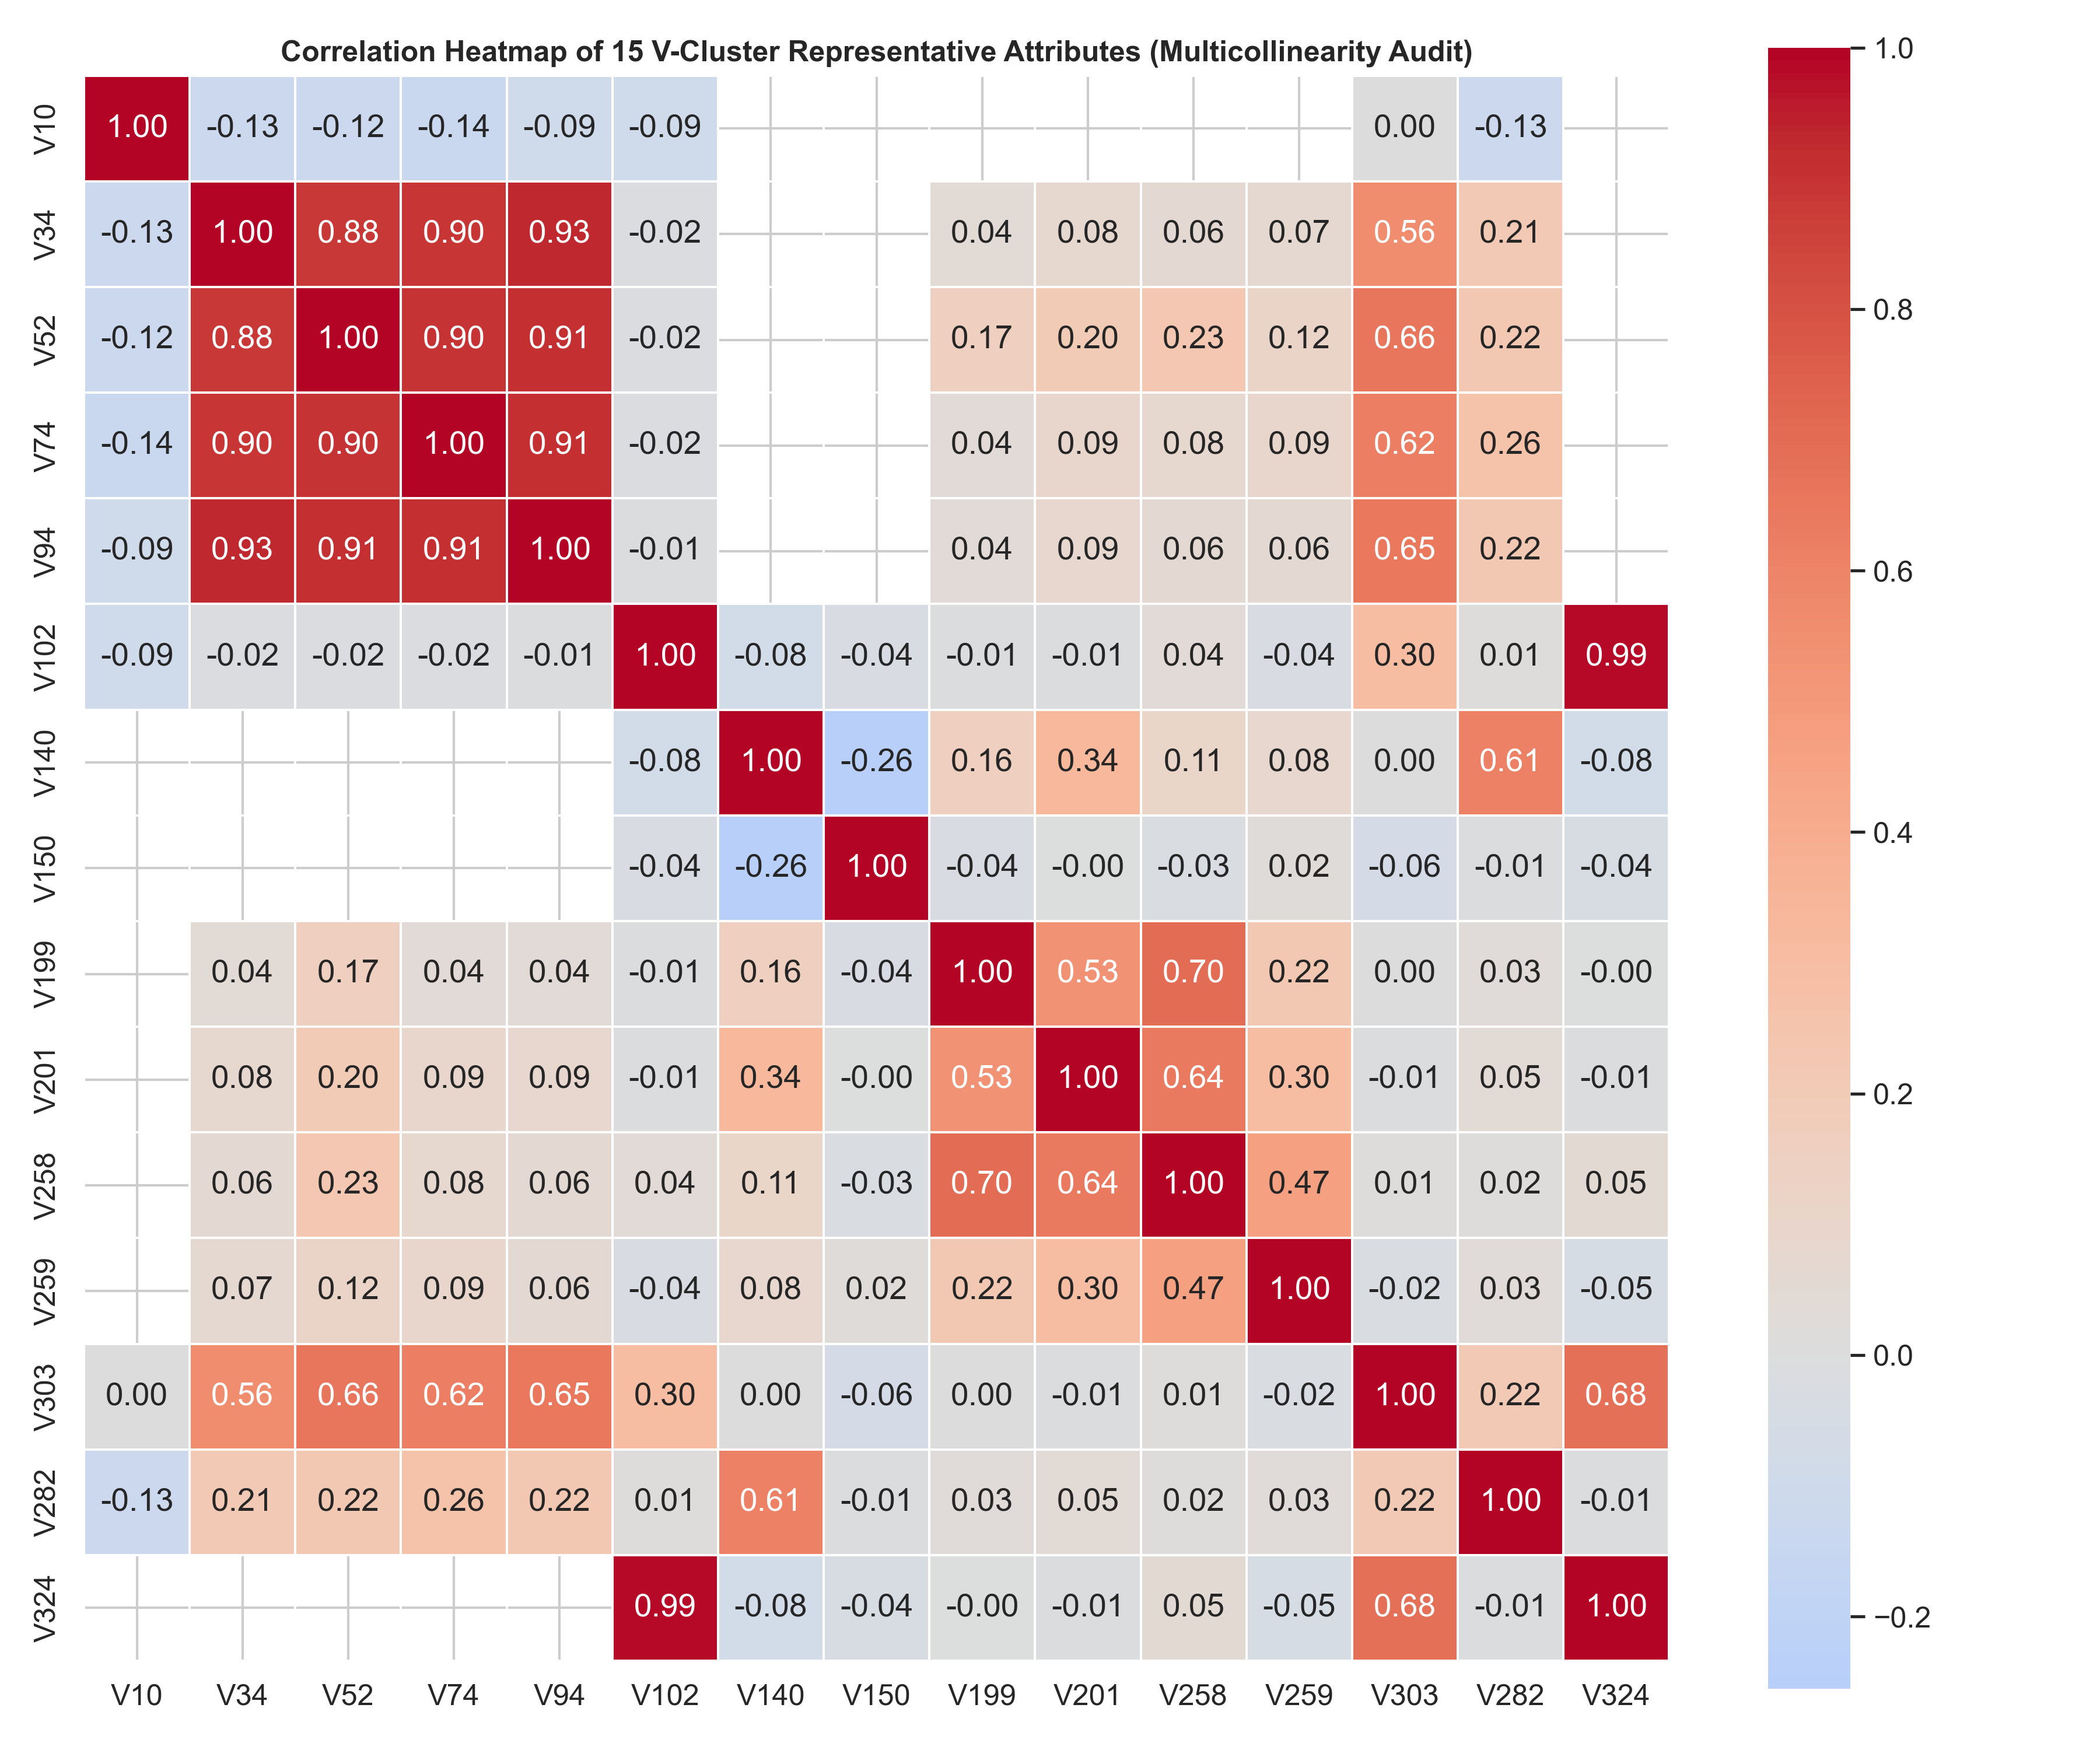
\includegraphics[width=0.95\linewidth]{../outputs/figures/v_cluster_heatmap.png}
\caption{Cross-correlation heatmap of the 15 V-cluster representatives, confirming reduced multicollinearity across independent clusters.}
\label{fig:v_heatmap}
\end{figure}

Fig.~\ref{fig:v_heatmap} validates that between-cluster correlations remain moderate to low, effectively eliminating the pathological collinearity that degrades gradient descent.

% =============================================================================
% 5. DEEP TABULAR ARCHITECTURE & METHODOLOGY
% =============================================================================
\section{Deep Tabular Architecture \& Implementation}
Building on these empirical foundations, we implemented a vectorized preprocessing and deep tabular neural pipeline.

\subsection{Entity Embedding Formulation}
For each categorical attribute $i \in \{1, \dots, 49\}$ with cardinality $K_i$, an embedding matrix $\mathbf{E}_i \in \mathbb{R}^{K_i \times d_i}$ projects discrete tokens into dense latent vectors:
\begin{equation}
\mathbf{z}_i = \mathbf{E}_i(x_i), \quad d_i = \min\left(50, \left\lfloor \frac{K_i^{0.5}}{2} \right\rfloor + 2\right)
\end{equation}
Out-of-vocabulary categories in the out-of-time validation or test sets are mapped to an explicit unseen token index $K_i$, preventing indexing crashes during inference.

\subsection{Numerical Preprocessing}
Continuous attributes undergo non-linear stabilization:
\begin{itemize}
    \item $TransactionAmt$ and transaction velocity counters $C1-C14$ undergo logarithmic transformation $\log(1 + \max(x, 0))$ to quell severe right skewness.
    \item Timedelta intervals $D1-D15$ are zero-clipped to suppress clock drift artifacts.
    \item Train-set medians impute missing values, followed by Standard Normal scaling $(\mu=0, \sigma=1)$ fitted strictly on training data.
\end{itemize}

\subsection{Focal Loss Objective}
To counteract the 27.5:1 imbalance between legitimate and fraudulent transactions without artificially distorting mini-batch distributions through oversampling, the model optimizes a numerically stabilized Binary Focal Loss:
\begin{equation}
\mathcal{L}_{\text{Focal}}(p_t) = -\alpha_t (1 - p_t)^\gamma \log(p_t)
\end{equation}
with $\alpha = 0.25$ and $\gamma = 2.0$. The modulating factor $(1 - p_t)^\gamma$ automatically suppresses the loss contribution from easily classified negative transactions, allowing gradients to focus on hard fraud instances.

% =============================================================================
% 6. CONCLUSION & REPRODUCIBILITY
% =============================================================================
\section{Conclusion \& Repository Artifacts}
This work delivers a rigorous, leakage-free empirical foundation for fraud detection on high-dimensional financial data. By resolving 49 entity attributes, reverse-engineering hardware signals, clustering 339 $V$-features into 15 orthogonal representations, and establishing a strict chronological partition, the pipeline eliminates critical points of failure.

All code modules (`src/config.py`, `src/preprocess.py`, `src/dataset.py`, `src/losses.py`, `src/models.py`, `src/train.py`, `src/evaluate.py`, `src/run_experiments.py`), preprocessed Parquet datasets, and statistical diagnostic evidence (`outputs/`) are structured for reproducibility and git repository deployment.

% =============================================================================
% REFERENCES
% =============================================================================
\begin{thebibliography}{00}
\bibitem{ieeecis} IEEE Computational Intelligence Society, ``IEEE-CIS Fraud Detection Benchmark,'' Kaggle Competition, 2019. \url{https://www.kaggle.com/c/ieee-fraud-detection}
\bibitem{entity_embeddings} C. Guo and F. Berkhahn, ``Entity Embeddings of Categorical Variables,'' \textit{arXiv preprint arXiv:1604.06737}, 2016.
\bibitem{tabnet} S. O. Arik and T. Pfister, ``TabNet: Attentive Interpretable Tabular Learning,'' in \textit{Proc. AAAI Conf. on Artificial Intelligence}, vol. 35, no. 8, pp. 6679--6687, 2021.
\bibitem{focalloss} T.-Y. Lin, P. Goyal, R. Girshick, K. He, and P. Dollár, ``Focal Loss for Dense Object Detection,'' in \textit{Proc. IEEE Int. Conf. on Computer Vision (ICCV)}, pp. 2980--2988, 2017.
\bibitem{leakage} S. Kapoor and A. Narayanan, ``Leakage and the Reproducibility Crisis in Machine-Learning-Based Science,'' \textit{Patterns}, vol. 4, no. 9, p. 100804, 2023.
\end{thebibliography}

\end{document}
